%\section{Tulokset}
\section{Analysis of the proposed antennas}
\label{sec:analysis}
In the previous section, the results are only explained, and based on them some conclusions are made for the next simulation round. This section provides more thorough analysis on the results, and in the structure itself. The designed antennas are analyzed by both technical and general aspects. Last part of this section discusses possible improvements for this structure.

\vspace{-7pt}
\subsection{Fulfillment of objectives}
\label{sec:fulfillment}
\vspace{-3pt}
In this thesis, it is defined to design two cellular antennas to operate on both $704-960\,\mega\hertz$ and $1.71-2.69\,\giga\hertz$ frequency ranges. Additionally, two antennas to support GPS and Wi-Fi connections should be designed. Moreover, each antenna should be matched to $-5\,\db$, and have a certain efficiency. The minimum efficiencies are $30\,\%$ for cellular and $40\,\%$ for other antennas. Also, the isolation between the two cellular antennas should be at least $-15\,\db$.

The final structure indeed has all four required antennas, which are all performing quite well. Obtaining the desired matching level is the most problematic part, and as is seen in the results, the target mostly is not reached. The best matching levels are achieved in the $5\,\giga\hertz$ Wi-Fi band. However, as it is explained earlier, worse matching is accepted if efficiency target is reached. As the efficiency results show, those targets are reached by cellular antennas, and nearly reached by other antennas. The efficiencies are calculated with (\ref{eq:eff_aprx}), and thus it must be remembered that the results are only approximations. They can be anyway considered quite accurate as the only lossy parts of the simulation model are the plastic rim and the matching components. 

The only antenna not reaching the efficiency target is Element 7 at $2.4\,\giga\hertz$ Wi-Fi band, having the peak efficiency only a little above the target. However, this probably would not be a problem if this antenna was used in a consumer product, as the other Wi-Fi antenna is working fine, and also the performance of the cellular antennas is good at that frequency range. If needed, one of the cellular antennas could be used also for WLAN communications. The GPS antennas, on the other hand, have proper efficiencies, but their bands are a little too narrow. Fortunately, the whole GPS band is covered as the operating frequencies of the two antennas slightly overlap.

Besides efficiencies, also the isolation of cellular antennas is under interest. As it is presented, the two ends of the phone are not interfering with each other, as the target isolation is reached for all elements at all operating frequencies. A little negative discovery is the internal isolation of both main and diversity antenna. Those do not have any target but the isolations are not that good, which is seen as decreased efficiency, especially for the diversity antenna. Even though it is desired that the antenna elements couple strongly, power should not flow to the ports of other elements. However, as the efficiencies are good, this is not a major problem.

Generally, the design objectives are fulfilled very well, and the antennas are operating as desired. Of course, the performance can always be improved, which is discussed further in Subsection \ref{sec:improvements}.


\subsection{General discussion}
\label{sec:general_discussion}
Besides analyzing the accomplished objectives, the results of this project should be compared to previous studies, and have its advantages and drawbacks evaluated.

One significant difference between this project and all the earlier presented, previously published papers is the simulation model. As far as the author knows, using as realistic model as this one is not reported. This increases the value of these obtained results, as they might correspond better to the consumer products. However, the realistic model is also a drawback, and complicates the research process. Constructing a prototype is much harder, and the matching circuits with several components are not making it easier. Measuring a prototype antenna is an important part of the design process to confirm the simulation results, and also to see if the structure is realizable.

The designed structure has a few clear advantages. The first one is the back cover. Only two of the most recent studies have a solid and slotless back cover. Typically at least one slot or opening is used to enhance radiation and simplify the problem. For this thesis, it is described to use a cover without any discontinuities. This detail together with the accuracy of the simulation model makes the environment and the case completely different to previous studies for this project, which gives a major advantage for further studies. 

Secondly, using the side metals as antennas is not a new idea, but it is a general advantage, as that technique frees up the already limited space inside the phone for other subsystems. However, as the antennas are integrated to the sides, it makes the rim broken several times. This might be bad for the robustness of the phone compared to the strength of an unbroken rim. Also, the antenna elements themselves are quite large, which is fine due to the structural integration, but in case of an impact, they might be more likely to become damaged.

The performance of this designed system is competitive against the previous studies, regardless of the structural differences of the models. The most remarkable detail is the frequency band, which in this case starts from 704 MHz. Only a couple of the earlier studies support that low frequencies. The cellular efficiencies of the designed antennas are at range $30-60\,\%$, which is about the same as other previously studied metal-covered handsets have.


\subsection{MIMO capability}
\label{sec:mimo_cap}
In a modern mobile phone, it is common to have multiple antennas for the same frequencies, i.e.\ to support MIMO techniques. In this project, it is defined to have MIMO capability at cellular frequencies. This is also a clear advantage over the previously studied antennas, as only a few of them are capable of MIMO communications. The simulation results presented in Section \ref{sec:complete_structure} show that the main and the diversity antenna both reach the efficiency target easily. As the structure does not have any tuners or switches, these two antennas are able to communicate simultaneously. Also, the antennas are well isolated, and thus they should not interfere with each other.

As Section \ref{sec:multiant} explains, envelope correlation coefficient can be used to evaluate MIMO capability of a mobile phone besides efficiency, matching, or isolation. EEC is calculated for both the low and the high band with (\ref{eq:ecc}). Again, as this structure has some losses in the plastic rim and matching components, the calculated value will only result an approximation of the coefficient, which is seen in Figure \ref{fig:ecc}. 
\begin{figure}[H]
    \centering
    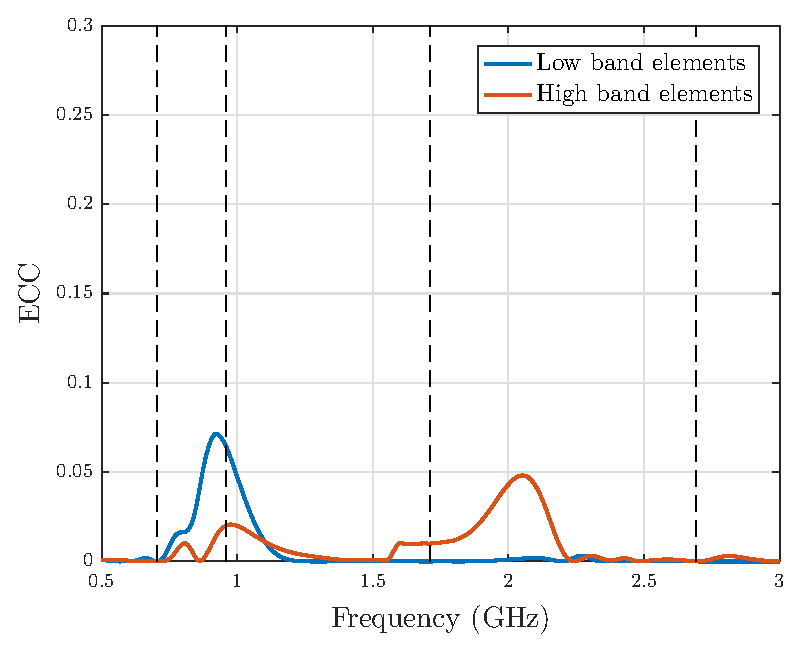
\includegraphics[width=0.5\textwidth]{img/ecc.eps}
    \caption{Envelope correlation coefficient for low and high cellular bands.}
    \label{fig:ecc}
\end{figure}

The ECC curves confirm the observations from the other results. Generally, $\rho_e\leq0.5$ is considered as good performance, and in this case the ECC is clearly below 0.1 in both bands. Moreover, the correlation is near 0 for the most of the operating bands, meaning the two antennas are completely uncorrelated. Therefore the MIMO capability of this design is remarkably good, as the antennas are radiating well and not negatively affecting each other.

\subsection{Possible improvements \& future work}
\label{sec:improvements}
Even though the proposed design performs well, the system can still be improved. The next main step would be constructing a prototype to confirm the simulation results. In order to do that and realize the design, one major challenge is the matching circuitry. Although the networks are simplified a lot, the topologies still have rather many components. With fewer components it is easier to control the performance, and realizing the design becomes significantly simpler. Possible solutions for this would be for example tunable capacitors. Using DTCs would not necessarily improve the overall performance, but matching circuits might operate decently with fewer components. In order to use DTCs, the current matching networks would require a complete reconstruction. Other way could be to investigate further the Topology 1 proposed in Section \ref{sec:sim_realistic}, and see if that design could be simplified. By looking the proposed component values, it does not seem to be impossible to have only one feeding port and two reactively loaded elements. This would notably decrease the number of matching components, which clearly would be an improvement. In that case, only one element would radiate, which might yield slightly decreased performance due to the large frequency range to cover, but the system would be much simpler.

Changes in the actual antenna structure should also be considered, if other solutions are not helping. One potential structure would be having multiple feeds on one single element, like is proposed in \cite{valkonen_multifeed}. In that design, each feed is matched for some frequency band, and that way one element radiates at all desired frequencies. The antenna in that paper, however, is not tested in metal-covered phone, which makes it worth trying a similar design.

Minor modifications would consider the appearance of the phone, if a consumer product was manufactured. Of course the simulation model is quite harsh, and the actual phone would look nicer, but the antenna design has some visually unappealing details. For example the gaps between different antennas are not constant and are located non-symmetrically. This small matter should be investigated, since even the smallest dimensional changes might affect a lot on antenna's performance, as it is seen in the simulations.

Maybe the most significant disturbance, which is not studied in this thesis, is the hand-effect. Mobile phones are mainly kept in hands when used and also located very close to the user's head when a call is on-going. This effect is studied widely, and also included in many of the papers referenced in Section \ref{sec:metal_cover}. The simulation model used in this project is already challenging due to the metallic back cover and other parts of the phone that are modeled as metal blocks, and adding user's hand or head to this environment would complicate the simulations a lot. That is anyway an important detail to test due to the fact that phones are mainly used in a close proximity of a person. Without researching that effect, it is impossible to tell for sure if the designed structure is actually usable in practice.


\clearpage